\documentclass[border=5pt]{standalone}
\usepackage[T1]{fontenc}
\usepackage{tikz}
\usepackage{amsmath,amssymb}
\usetikzlibrary{positioning, arrows.meta, fit, backgrounds, calc, decorations.pathreplacing}

% === Color palette ===
\definecolor{cBlue}{HTML}{3B7DD8}
\definecolor{cOrange}{HTML}{E07B39}
\definecolor{cPurple}{HTML}{8E44AD}
\definecolor{cGray}{HTML}{5D6D7E}

\begin{document}
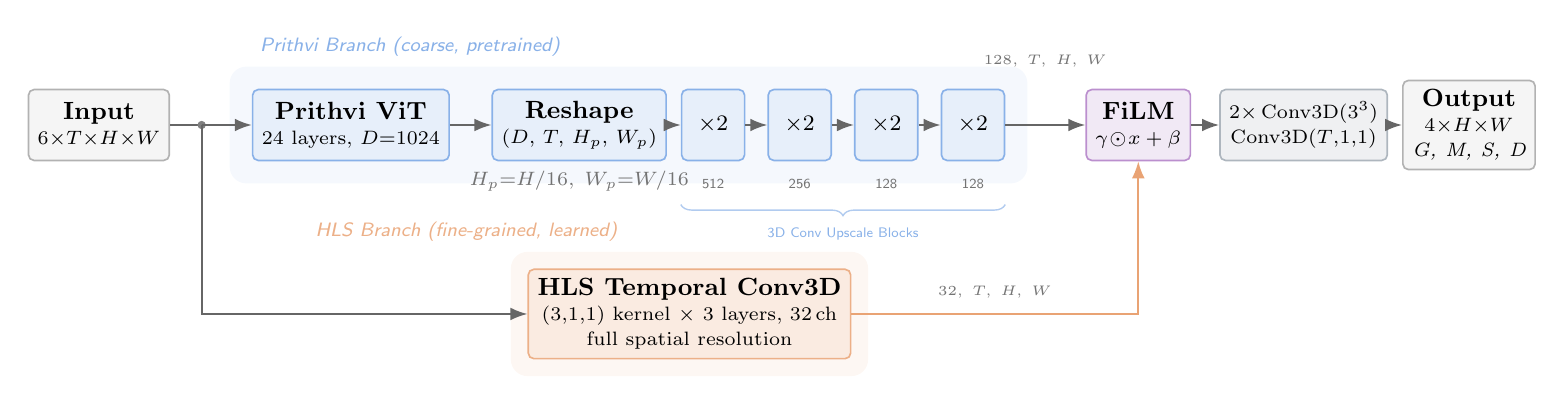
\begin{tikzpicture}[
    >=Latex,
    % --- Node styles ---
    block/.style={
        draw, rounded corners=2pt, minimum height=0.9cm,
        align=center, font=\small, line width=0.6pt
    },
    pb/.style={block, fill=cBlue!12, draw=cBlue!60},
    hb/.style={block, fill=cOrange!15, draw=cOrange!60},
    fb/.style={block, fill=cPurple!12, draw=cPurple!60},
    gb/.style={block, fill=cGray!10, draw=cGray!50},
    io/.style={block, fill=black!4, draw=black!30},
    % --- Arrow styles ---
    arr/.style={->, line width=0.7pt, draw=black!60},
    harr/.style={->, line width=0.7pt, draw=cOrange!70},
    % --- Annotation styles ---
    shp/.style={font=\tiny\sffamily, text=black!55},
    brclabel/.style={font=\tiny\sffamily, text=cBlue!60},
]

% =============================================
% MAIN ROW (y=0): Prithvi path
% =============================================

\node[io, minimum width=1.6cm] (in) at (0, 0) {
    \textbf{Input}\\[-2pt]
    {\scriptsize $6{\times}T{\times}H{\times}W$}
};

\node[pb, minimum width=2.2cm] (enc) at (3.2, 0) {
    \textbf{Prithvi ViT}\\[-2pt]
    {\scriptsize 24 layers, $D{=}1024$}
};

\node[pb, minimum width=1.4cm] (resh) at (6.1, 0) {
    \textbf{Reshape}\\[-2pt]
    {\scriptsize $(D,\, T,\, H_p,\, W_p)$}
};

% Upscale blocks
\node[pb, minimum width=0.8cm] (u1) at (7.8, 0)  {\footnotesize $\times$2};
\node[pb, minimum width=0.8cm] (u2) at (8.9, 0)  {\footnotesize $\times$2};
\node[pb, minimum width=0.8cm] (u3) at (10.0, 0) {\footnotesize $\times$2};
\node[pb, minimum width=0.8cm] (u4) at (11.1, 0) {\footnotesize $\times$2};

% FiLM — extra horizontal room for shape label
\node[fb, minimum width=1.3cm] (film) at (13.2, 0) {
    \textbf{FiLM}\\[-2pt]
    {\scriptsize $\gamma \!\odot\! x + \beta$}
};

% Temporal Fusion Head — show actual conv operations
\node[gb, minimum width=1.8cm] (head) at (15.3, 0) {
    {\scriptsize $2{\times}$\,Conv3D$(3^3)$}\\[-2pt]
    {\scriptsize Conv3D$(T{,}1{,}1)$}
};

% Output
\node[io, minimum width=1.5cm] (out) at (17.4, 0) {
    \textbf{Output}\\[-2pt]
    {\scriptsize $4{\times}H{\times}W$}\\[-2pt]
    {\scriptsize\itshape G, M, S, D}
};

% =============================================
% HLS BRANCH (below main row)
% =============================================

\node[hb, minimum width=4.0cm] (hls) at (7.5, -2.4) {
    \textbf{HLS Temporal Conv3D}\\[-2pt]
    {\scriptsize $(3{,}1{,}1)$ kernel $\times$ 3 layers, 32\,ch}\\[-2pt]
    {\scriptsize full spatial resolution}
};

% =============================================
% ARROWS
% =============================================

% Fork point from input
\coordinate (fork) at ($(in.east) + (0.4, 0)$);
\draw[line width=0.7pt, draw=black!60] (in.east) -- (fork);
\fill[black!50] (fork) circle (1.5pt);

% Fork to Prithvi encoder (straight right)
\draw[arr] (fork) -- (enc.west);

% Fork to HLS branch (down then right)
\draw[arr] (fork) |- (hls.west);

% Prithvi internal path
\draw[arr] (enc) -- (resh);
\draw[arr] (resh) -- (u1);
\draw[arr] (u1) -- (u2);
\draw[arr] (u2) -- (u3);
\draw[arr] (u3) -- (u4);
\draw[arr] (u4) -- (film);

% HLS to FiLM (right then up)
\draw[harr] (hls.east) -| (film.south);

% FiLM to Head to Output
\draw[arr] (film) -- (head);
\draw[arr] (head) -- (out);

% =============================================
% TENSOR SHAPE ANNOTATIONS
% =============================================

% Channel dims under each upscale block
\node[shp, below=3pt of u1] {512};
\node[shp, below=3pt of u2] {256};
\node[shp, below=3pt of u3] {128};
\node[shp, below=3pt of u4] {128};

% After upscaler, before FiLM — centered in the gap
\node[shp] at ($(u4.north east)!0.5!(film.north west) + (0, 0.35)$) {
    $128,\; T,\; H,\; W$
};

% HLS output shape (on the horizontal segment of the L-shaped arrow)
\node[shp, above=2pt] at ($(hls.east)!0.5!(hls.east -| film.south)$) {
    $32,\; T,\; H,\; W$
};

% =============================================
% BRACE: label the upscale blocks
% =============================================

\draw[
    decorate,
    decoration={brace, mirror, amplitude=4pt},
    line width=0.5pt,
    draw=cBlue!40
]
    ($(u1.south west) + (0, -0.55)$) -- ($(u4.south east) + (0, -0.55)$)
    node[midway, below=5pt, brclabel] {3D Conv Upscale Blocks};

% Patch size note under reshape
\node[shp] at ($(resh.south) + (0, -0.25)$) {
    {\scriptsize $H_p{=}H{/}16,\; W_p{=}W{/}16$}
};

% =============================================
% BACKGROUND SHADING for branches
% =============================================

\begin{scope}[on background layer]
    % Extra vertical padding so shape labels don't clip the background edge
    \node[
        fill=cBlue!5, rounded corners=6pt, inner sep=8pt,
        fit=(enc)(resh)(u1)(u2)(u3)(u4),
        label={[font=\scriptsize\sffamily, text=cBlue!60]above left:{\itshape Prithvi Branch (coarse, pretrained)}}
    ] {};
    \node[
        fill=cOrange!6, rounded corners=6pt, inner sep=6pt,
        fit=(hls),
        label={[font=\scriptsize\sffamily, text=cOrange!60]above left:{\itshape HLS Branch (fine-grained, learned)}}
    ] {};
\end{scope}

\end{tikzpicture}
\end{document}
